\section{Application in Circuit Analysis}

\begin{frame}{Application: MOSFET Amplifier}
    \begin{figure}
        \centering
        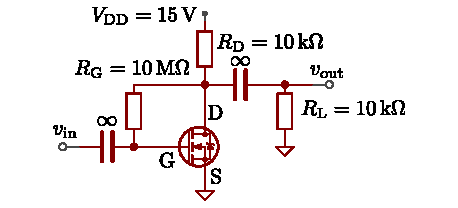
\includegraphics{../assets/example_circuit_small.pdf}
        \caption{MOSFET amplifier circuit.}
        \label{fig:mosfet_amplifier}
    \end{figure}

    What is the amplification $v_\mathrm{out}/v_\mathrm{in}$ of this amplification circuit?
    \begin{enumerate}
        \item Identify DC operating point
        \item Replace MOSFET with small signal model, analyze small signal circuit
        \item Sum DC and AC contributions
    \end{enumerate}
\end{frame}
\note[itemize]{
    \item DC operating point: circuit state with only DC signals
}

\begin{frame}{Application: DC Operating Point}
    \begin{itemize}
        \item Replace AC sources with short circuits
        \item Large capacitors act as open circuits for DC signals
    \end{itemize}
    \begin{figure}
        \centering
        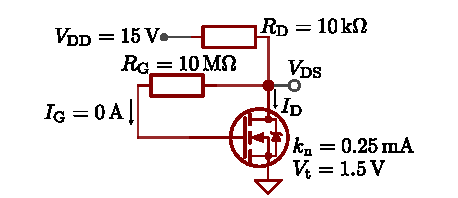
\includegraphics{../assets/example_circuit_dc.pdf}
        \caption{Reduced amplifier circuit, DC operating point.}
        \label{fig:mosfet_amplifier_dc}
    \end{figure}
    \begin{align*}
        I_{\mathrm{D}}&=\frac{1}{2}k_{\mathrm{n}}(V_{\mathrm{GS}}-V_{\mathrm{T}})^{2} 
        = \qty{1.06}{\milli \ampere}\\
        V_{\mathrm{GS}}&=V_{\mathrm{DS}}=V_{\mathrm{DD}}-R_{\mathrm{D}}I_{\mathrm{D}}
        =\qty{4.4}{\volt} \\
        g_\mathrm{m} &= k_\mathrm{n} (V_\mathrm{GS}-V_t) = \qty{0.725}{\milli \ampere \per \volt}
    \end{align*}
\end{frame}

\begin{frame}{Application: Small Signal Replacement}
    \begin{itemize}
        \item Replace DC sources with short circuits
        \item Large capacitors act as short circuits for high frequency signals
        \item Simplify circuit using linear circuit analysis
    \end{itemize}
    \begin{figure}
        \centering
        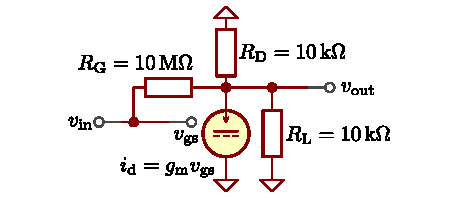
\includegraphics{../assets/mosfet_amplifier_small_signal.pdf}
        \caption{Reduced amplifier circuit, small signal model.}
        \label{fig:mosfet_amplifier_ac}
    \end{figure}
\end{frame}

\begin{frame}{Application: Small Signal Analysis}
    \begin{itemize}
        \item Simplify circuit by combining both resistors
    \end{itemize}
    \begin{figure}
        \centering
        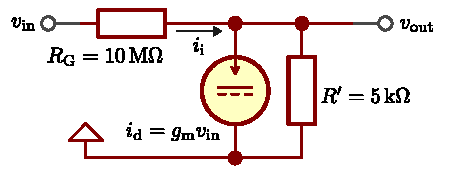
\includegraphics{../assets/mosfet_amplifier_small_signal_reduced.pdf}
        \caption{Reduced amplifier circuit, small signal model.}
        \label{fig:mosfet_amplifier_ac_2}
    \end{figure}

    \begin{align*}
        R'=R_\mathrm{D} \parallel R_\mathrm{L} &= \qty{5}{\kilo \ohm} \\
        v_{\mathrm{in}}-v_{\mathrm{out}}&=R_{\mathrm{G}} i_{\mathrm{i}} \\
        (g_{\mathrm{m}}v_{\mathrm{gs}})+v_{\mathrm{out}} /R'&=i_{\mathrm{i}}
    \end{align*}
\end{frame}

\begin{frame}{Application: Small Signal Analysis}
    \begin{figure}
        \centering
        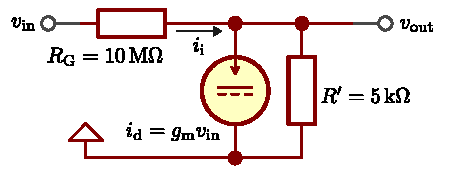
\includegraphics{../assets/mosfet_amplifier_small_signal_reduced.pdf}
        \caption{Reduced amplifier circuit, reduced small signal model.}
        \label{fig:mosfet_amplifier_ac_reduced}
    \end{figure}
    \begin{itemize}
        \item Solve for the amplification:
    \end{itemize}
    \begin{align*}
        v_{\mathrm{in}}-v_{\mathrm{out}}&=R_{\mathrm{G}}\left( g_{\mathrm{m}}v_{\mathrm{in}}+\frac{v_{\mathrm{out}}}{R'} \right) \\
        v_{\mathrm{out}}\left( -1-\frac{R_{\mathrm{G}}}{R'} \right)&=v_{\mathrm{in}}(-1+R_{\mathrm{G}}g_{\mathrm{m}}) \\
        \frac{v_{\mathrm{out}}}{v_{\mathrm{in}}}&=\frac{1-R_{\mathrm{G}}g_{\mathrm{m}}}{1+R_{\mathrm{g}} / R'}=\num{-3.6}
    \end{align*}
\end{frame}